\section{Comparação do fluxo da Requisição}

    \par O fluxo da Arquitetura MVC Original, ilustrado na Figura~\ref{fig:mvc1}, é direto e revela um alto nível de acoplamento ao \textit{framework}, violando o Princípio da Responsabilidade Única. A requisição HTTP (\texttt{POST /contacts}) é recebida pela Rota, que a encaminha ao \texttt{ContactController}. O \textit{Controller} é então ativado e assume múltiplas responsabilidades simultaneamente: ele instancia diretamente o \texttt{ContactModel} (Eloquent), criando um forte acoplamento ao ORM, e define seus atributos com os dados brutos da requisição HTTP. 
    
    \par Em seguida, o \textit{Controller} chama o método \texttt{save()} do \textit{Model}, orquestrando a persistência de dados no Banco de Dados. Esse comportamento fez com que o \textit{Controller} atue como manipulador de HTTP, orquestrador de lógica de negócio e componente de acesso a dados. O fluxo é finalizado com o \textit{Controller} retornando a resposta JSON ao Cliente, acumulando também a responsabilidade de formatação da saída (\textit{Presenter}).

    \par Com a refatoração, o fluxo (Figura~\ref{fig:ca1}) inverte as dependências, garantindo que o núcleo da aplicação seja totalmente isolado. O processo começa com o \texttt{Controller} (Adaptador de Interface) recebendo a requisição HTTP (1). Seu papel é estritamente limitado à tradução da entrada: ele cria o \texttt{RequestModel} (DTO) (2) e invoca o Caso de Uso através da interface \texttt{InputBoundary} (3), passando o DTO agnóstico e uma instância do \texttt{Presenter}.

    \par O \texttt{Interactor} (Caso de Uso) é ativado na camada de lógica de negócio. Sua responsabilidade é puramente a execução da regra: ele cria e valida a \texttt{Entidade Contact} (4) e, para persistir, chama a \texttt{ContactRepositoryInterface} (5). A Regra da Dependência é estritamente obedecida, pois o \textit{Interactor} não conhece o \textit{framework} ou o ORM. A implementação concreta do repositório interage com o Banco de Dados (6, 7, 8) e retorna a \texttt{Entidade Salva} para o \textit{Interactor}.

    \par O \texttt{Interactor} cria o \texttt{ResponseModel} (DTO de saída) (9) e o envia ao \texttt{Presenter} através da \texttt{OutputBoundary} (10), finalizando a lógica de negócio. O \texttt{Presenter} (Adaptador de Saída) formata os dados brutos no \texttt{ViewModel} (11). O \texttt{Controller} (Adaptador de Entrada) recupera o \texttt{ViewModel} (13, 14) e envia a resposta JSON (15). Essa segregação de tarefas, ao isolar a lógica de negócio na camada de \textit{Use Cases}, torna o núcleo da aplicação totalmente testável em unidade (sem dependência do \textit{framework}, \textit{HTTP} ou Banco de Dados) e flexível a alterações de tecnologia externa.

    \begin{figure}[H]
        \centering
    
        \begin{minipage}{0.49\linewidth}
            \centering
            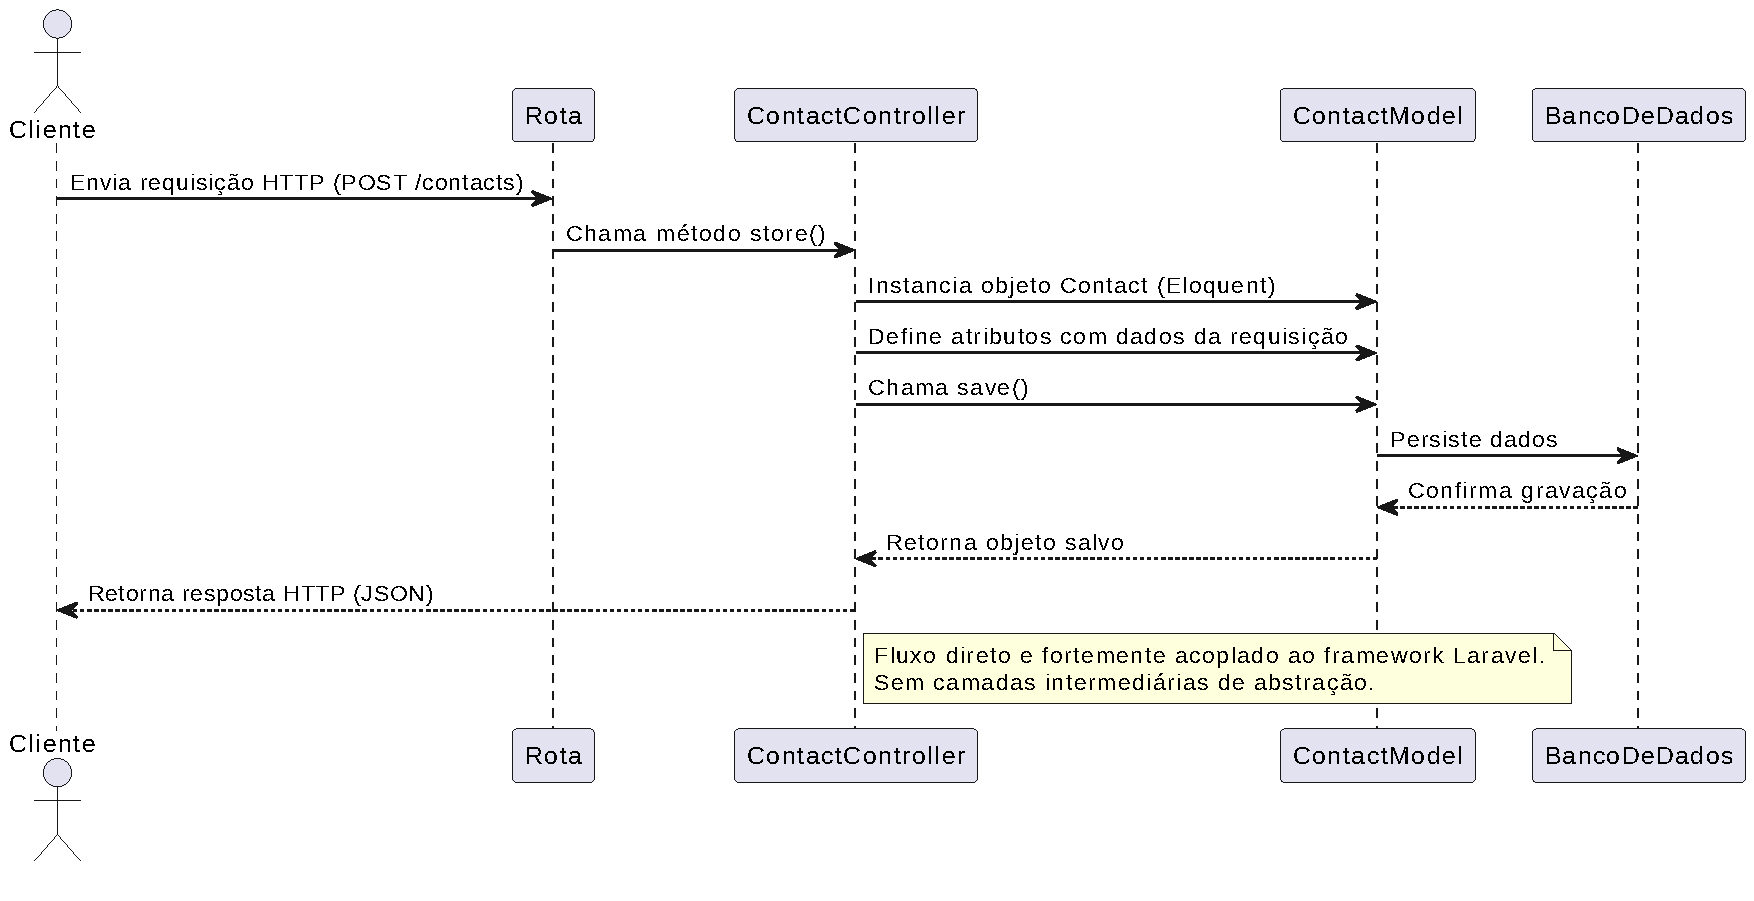
\includegraphics[angle=-90,width=1.0\linewidth]{figuras/resultados/mvc1.pdf}
            \caption{Fluxo da Requisição - Arquitetura MVC Original (Laravel).}
            \label{fig:mvc1}
            
        \end{minipage}
        \hfill
        \begin{minipage}{0.49\linewidth}
            \centering
            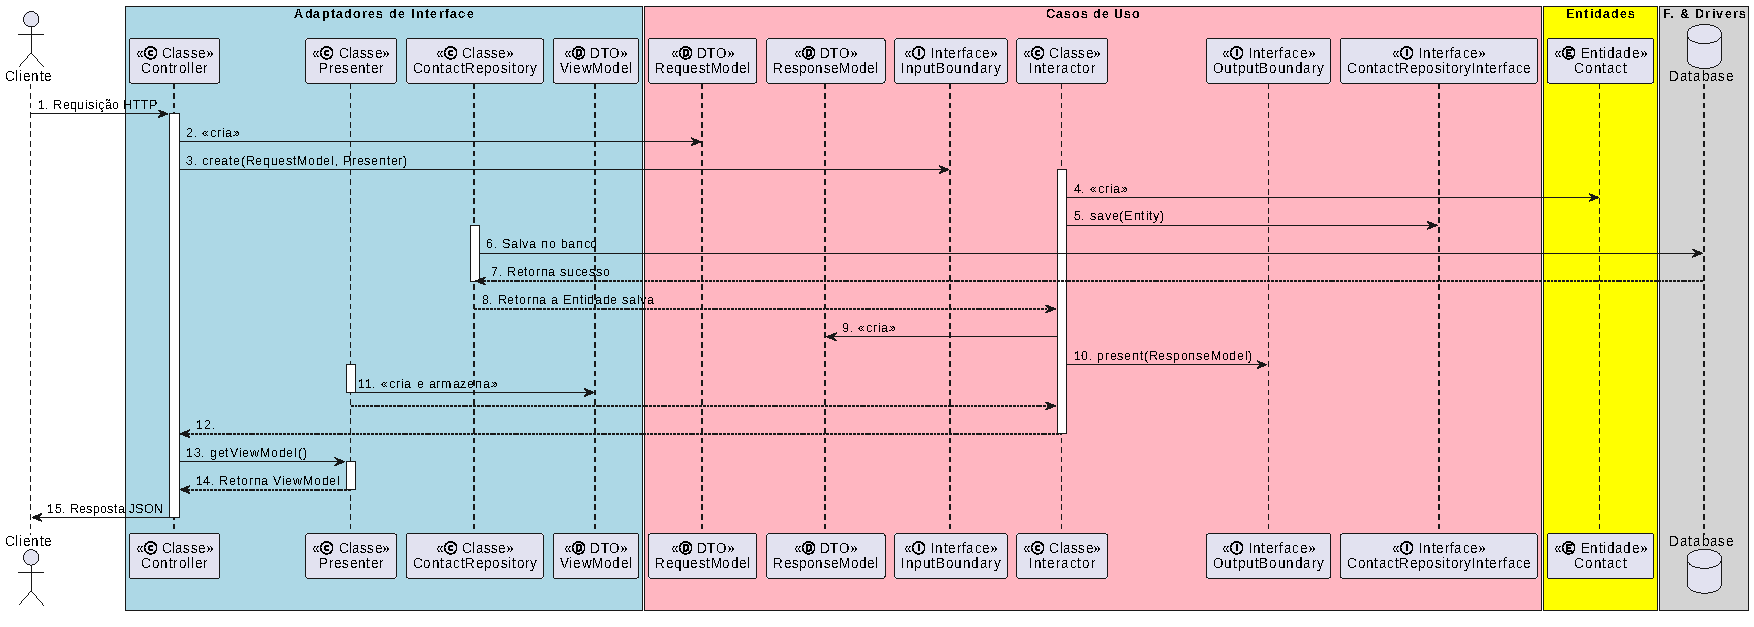
\includegraphics[angle=-90,width=1.0\linewidth]{figuras/resultados/ca1.pdf}
            \caption{Fluxo da Requisição - Arquitetura Limpa (Laravel).}
            \label{fig:ca1}
            
        \end{minipage}
    \end{figure}

    \vspace{1cm}
